\chapter{Methods}

The implementation efforts of this thesis are condensed into the following chapter. A holistic perspective on the data process is described in the following step following from the urgency that Sensor Health Monitoring needs to be perceived within its ecosystem. A SHM thus is directly reliant upon the data in the first place. It is then also reliant upon the configuration metadata since it will contain necessary information for processing the data further within the SHM. To then close the feedback loop it is also vital to generate a sensible data display that allows quick evaluation of the SHM since manual evaluation methods would slow the development process by orders of magnitude.


\section{Introduction}


The implementation can be detailed by figure \ref{fig:fti_microservices}. After having uploaded the Dataset the relevant information on the sensors as well as the aircraft properties is gathered and condensed into a single configuration metadata-set represented by a JSON file. This JSON file is then appended to the Dataset within the skystash architecture represented by the Online side that is accessed by the API. Processing the data now becomes a clean blackbox operation that is only fed by data received by the API returning its report containing notable occurences via the API and storing all relevant information online. Since this software is developed for flight operations and an interactive visualization of the report data facilitates evaluation of the generated report data a User Interface within a dashboard application is developed. Additional benefits contrary to the generation of PDF reports are dynamic updates as well as interactivity and an agile update cycle considering the spontaneous emergence of bugs.


\begin{figure}[h]
    \centering
    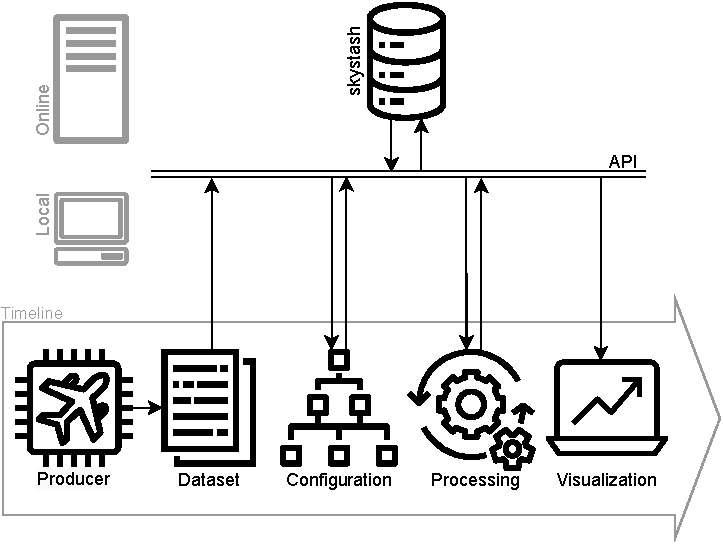
\includegraphics[width=.8\textwidth]{FT_microservices_AWS}
    \caption{The data toolchain prospectively used for Sensor Health Monitoring}
    \label{fig:fti_microservices}
\end{figure}


\section{Data Parsing}
Since the SHM has to run on something, the original data is briefly mentioned for completeness.

\subsection{ Parsing of ISTAR Data}

Istar data is parsed for each flight for each sensor. Istar config data is present for each flight in the shape of an imcexp file.

ISTAR data originates from the ISTAR's DAQ system in the shape of .raw files for each parameter and is parsed and uploaded to the stash. It is then accessible via the stash api and can also be inspected in the stash webview. After the Dataset generation step the metadata available is only the one from the ISTAR DAQ system.
The data is present in the shape of Projects->Collections->Series

The metadata is currently only the one from the ISTAR DAQ system. Since this metadata is not explicitly useful in itself it will be enriched further within the Configuration step (See figure \ref{fig:fti_microservices}).


\section{Configuration-Metadata}

get imcexp data
enrich excel data
-aircraft data
-shm data
-limits
-type
-tags
-reference COS
get excel data


generate merged view for metadata.


The metadata uploaded to the stash in itself is not very expressive and needs to be refined further into a usable, concise format. This step details the considerations and implementations taken to be able to generate a useful metadata model that applies necessary information to the dataset within the skystash.

\subsection{ Basics: Metadata Collection, formatting into SOIL}
The configuration of the ISTAR is of great importance for the data processing. Also of great importance is the knowledge database which is currently in the shape of an excel document.
Attributes that are generally transmitted within the DAQ configuration are sampling rates, data origins and other miscellaneous information related to the system. Not contained are information about general sensor description, position of sensors, overall setup of the aircraft sensor architecture and check limits for data values.

\subsection{Parsing and assignment of ISTAR data config}
-Additional Metadata
-physical limits
-amplitude limits
-tag (physical entity)
-reference ()


\section{Data Processing}

\subsection{Software architecture considerations}

Careful consideration needs to be given to the workflow of the level 1 check to allow scalability and minimal manual interaction in later stages. To achieve this architecture, manual steps are reduced as far as possible. However, some level of configuration must be implemented. Otherwise only relational sensor behaviour could be detected. Meaning that sensor faults occuring temporarily within an experiment can be detected but permanent behaviour is not noticed by a relative algorithm

\subsection{Check 1 Implementation}
For implementing the level 1 checks, the measured data needs to be compared to the expected data. To gain insight into what the the expected data is, the configuration file of the data acquisitioning system needs to get parsed.
Luckily, the DAQ's format is a .zip directory.
The 7zip command line tool gets used for opening the configuration file since the configuration file's format is not fully complying to the zip standard making several python libraries fail during the process. This stems from an issue with the zip header and footer parts of the file that are not at expected places (i.e.\ the front the back).
Once opened, the configuration file contains multiple files as well as an essential xml file that contains the needed sensor metadata.

Missing datasets can now easily be found by comparing the expected values from the configuration file to the actual generated data.

For the second step.

\subsubsection{All Parameters present?}

\subsection{Check 2 Implementation}
Since the IMC DAQ System resamples the 20Hz Sensors to a straight timeframe data gets lost in the process. This makes potentially noisy sensors output the same value twice in a row since the DAQ hasn't yet received the new sensor data and outputs the same value multiple times in a row. Even sensors with a high noise ratio such as the fine part of a gps latitude signal outputs the same value twice in a row which is highly unlikely to happen on a statistical basis. Since this occurs quite often the question arises if the actual sampling may be lower than the actual data.

\subsubsection{ No signal (value)}
A check implementation counterchecking the sensors sampling that generates fault detections based on deviation from predefined sampling. This takes into account the DAQ config since it contains the current sampling rate. Minimizing false positives.

\subsubsection{Out of range}
Generally, predefined limits are checked within SHM Level 2. For the first step, values are checked whether they are within a predefined range. This means e.g. a range of -1000-40000 ft for barometric altitudes. or 1Pa-120000Pa for static pressure ports. Of course, this selection is biased and may not be accurate for most mission profiles like atmospheric research aircraft that cruise in altitudes of up to 45,000 ft MSL.

\subsubsection{movement too high}
The next category examining the sensor behaviour can be classified into sensor movement being too low or sensor movement being too high. Movement being defined within this context as the difference of a new sensor value to the previous one. Of course, this topic could be examined within a depth that may exceed this work such as estimating white noise using discrete fourier Transform Subspace Decompositions \cite{hendriks_noise_2008} or statistical methods such as covariance operators.

The goal of this work however, is preservation of scalability, minimal user and configuration inputs. Hence, an approach using a STFT where the amplitude is averaged across all frequencies from its spectrum. This guarantees a generalized feature extraction, meaning standardization. Based on this spectral analysis, the logarithmic order of the variable can be estimated within its dataset. Previously, the frequency is assumed via time difference of start and end time divided by $n_{datapoints}$. The STFT also implements preprocessing steps that would otherwise be necessary such as translating the signal by its average value as well as scaling it by its standard deviation. Would one be interested in examining a signal using functions from a statistical toolbox, a similar result may be achieved by performing the previous steps of averaging and scaling the signal and then examining the variance within a moving window of the signal, similar to the STFT. The size of the moving window for such an analysis is defaulted to 256 data points for each signal. Certain issues with methods of moving windows are however, that they are not very meaningful for the beginning and ending of datasets within which the window is not fully occupied. This may lead to spikes for the STFT, which is why it is found that the STFT is generally more powerful to examine low sensor movement.

TODO: Comparison variance, standard deviation, mean noise. Scalability for other sensors.

Noise Tracking using DFT can be used to estimate noise combined with a strenuous effort
Since this however would exceed the scope of this work, a simpler algorithm is implemented by comparing moving window variance as well as STFT overall amplitude estimations.

Limits of variance and stdev.

To better approximate the errors concerning white noise, a STFT is employed.

White noise approximation methods. Rolling window variance.

\subsubsection{ movement too low}

\subsection{Check 3 Implementation: }

I lied about single source of config. Level 2 and 3 also have their own config.

avoid weighting by structuring checks into a tree format for independent aircraft state variables.


Aims of Level 3 Implementation are to model the aircraft's state in a reference system.
This reference system shall be geodetic and fixed to the earth while the aircraft moves through it. Moving aircraft coordinate systems like the aerodynamic and the along track Coordinate system may be derived from its geodetic position using ?angles and velocities.


Interfacing: Clean interfaces are generated throughout the model. Enabling a standardized state vector x. Meaning that A remains standardized for any aircraft while B, U and L need to be adjusted for any changes to the aircraft or sensor data.

The integration step may be omitted in early design stages since the necessary equations and equilibriums of Forces and Moments could only be modelled linearly while neglecting various unknown factors like shifting CG due to fuel burn, actual Inertia of Aircraft and aicraft mass. Hence, this step may be implemented if time allows it.

\subsubsection{Finding a reference state}

Necessary to compare parameters is a common reference system. Hence, reference systems are examined upon suitability for usage of parameter transformations.

A starting point which shall be considered is the geodetic reference.
it measures the aircraft's position by its displacement from the previously (ref?) discussed WGS84 system.
Meaning that altitude gets measured as the orthometric height (see ellipsoid height-geoid height).

Latitude and Longitude form the x and y axis of the COS. True heading forms the reference heading within the geodetic system.

All aircraft parameters related to motion and position of the aircraft should be attempted to be condensed into this form.

\paragraph{Dynamic configuration and correlation of parameters}

Motivation: a dynamic description for parameter correlations is searched in order to implement an efficient and quick way to assign parameter correlations. It is then assumed that a tree structure is fit for this task since parameters can be correlated to other upstream parameters in a single flow direction.


To attach meaning to the parameters, they are specifically tagged with descriptions of their function. A simple example that is implemented is that of \textit{static pressure}. The tag is defined in the excel configuration and furthermore gets configured into a dynamic configuration JSON-file. This file allows specification of sensors into subclasses and divides the aircraft into its degrees of freedom. This tree structure is then parsed and calculates a value for each level of detail taking into account its lower lying neighbours. Some weighting also has to be considered since a number of redundant pressure sensor could skew results against a single GNSS parameter. Thus a condensed parameter is calculated for each degree of freedom that is based on predefined algorithms and tags that can be freely defined within the config file that are then recursively parsed within the tree structure.

\begin{figure}
    \centering
    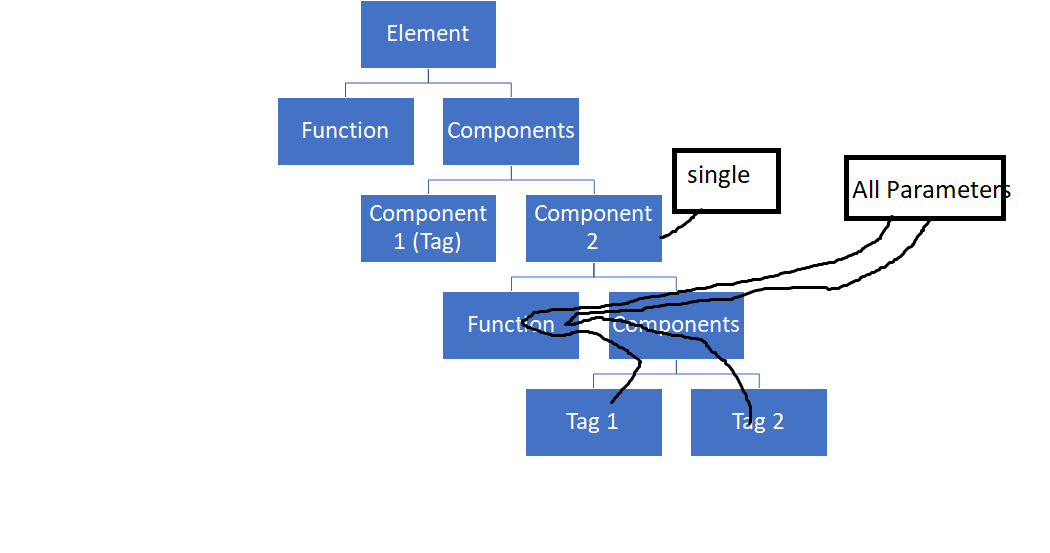
\includegraphics[width=\textwidth]{level3_config}
    \caption{General structure of physical correlation setup}
    \label{fig:level3_config}
\end{figure}


In figure \ref{fig:level3_config} the general structure of the dynamic configuration in JSON format is shown. The configuration parent is an element similar to the configuration in SOIL-format \cite{behrens_domain-specific_2021}. In our case the ISTAR-aircraft. The istar aircraft contains top-level components that are the independent state variables of the aircraft. Generally a component can contain other components or parameter tags that describe parameters that are referenced. A component can also contain a function that transforms its parameters into the parent parameter.

\paragraph{Residual generation}
Based upon this previously defined model that is based on the aircraft configuration as a tree structure, residuals are generated based upon the difference of the parameters to the top level parameters (Single, fused value) and the single transformed sensor values (All Parameters) as previously discussed in Table \ref{tab:states_and_signals}.


An alternate method for fusion of redundant sensors is proposed that is similar to voting algorithms employed by Flight Control Systems of \cite{tischler_advances_2018}. An issue for voting algorithms is the abrupt exclusion of single sensors once their difference to the other sensors is too large. Hence, a weighting strategy for averaging is proposed that is based on the value difference.

An example is shown in figure \ref{fig:fusing_method}

This method tries to account dynamically for sensor distance by scaling parameters to small values compared to their neighbours. This works for a minimum of three redundant values.

Based on the single sensor values a distance matrix for $d_{i,j}$ is set up.

% Please add the following required packages to your document preamble:
% \usepackage{booktabs}
\begin{table}[]
    \begin{tabular}{@{}llll@{}}
        \toprule
        & A    & B    & C    \\ \midrule
        \multicolumn{1}{l|}{A}   & 0    & 0.25 & 2    \\
        \multicolumn{1}{l|}{B}   & 0.25 & 0    & 1.75 \\
        \multicolumn{1}{l|}{C}   & 2    & 1.75 & 0    \\ \midrule
        \multicolumn{1}{l|}{Sum} & 2.25 & 2    & 3.75 \\ \bottomrule
    \end{tabular}
\end{table}

The column sum is then further defined $\hat{d_{i}}$. To generate a ratio we define:

\begin{equation}
    w_i=\frac{1}{\hat{d_i}}
    \label{eq:fusing_weight}
\end{equation}

Since we desire that
$\sum{w_i}\overset{!}{=}1$ we need to scale the ratios using:

\begin{equation}
    \bar{w_{i}} = \frac{w_i}{\sum{w_i}}
\end{equation}


With this ratio we can now calculate the new fused value:

\begin{equation}
    \bar{x} = \sum_{i}^{n} x_i \cdot \bar{w_{i}}
\end{equation}

This works out to a fused value that is shown in \ref{fig:fusing_algo}.

Compare results with averaging here using figure.

To further increase sensitivity for distance we can replace the term in equation \ref{eq:fusing_weight} with a quadratic term:
\begin{equation}
        w_i=\frac{1}{\hat{d_i}^2}
\end{equation}
\paragraph{Residual Interpretation}


The residuals are then checked against the limits of the standard deviation of the normal signal for a highpass filtering generated by taking a moving window of 256 points. If any value falls outside these values of the standard deviation of the condensed signal it is noted within the report. A fixed residual limit as well as a probability density function implemented in works such as \cite{svard_data-driven_2014} may be implemented at a later point.

\subsubsection{Examining Altitude Sensors}

As seen in~\ref{fig:gps_diff} gps altitudes have a base mean value of difference of about 3-4 meters. During flight level changes the base level changes significantly. Further investigation is needed how these changes may arise.

One possible approach would be considering different placements of gps antennas within the airframe. since the IMAR's position is precisely known and lies around the center of gravity but the ASCB's gps position is not known exactly the process is not facilitated. However using the process of lever arms the position could be roughly estimated and compensated from the altitude difference in figure \ref{fig:gps_diff}.

\begin{figure}[h]
    \centering
    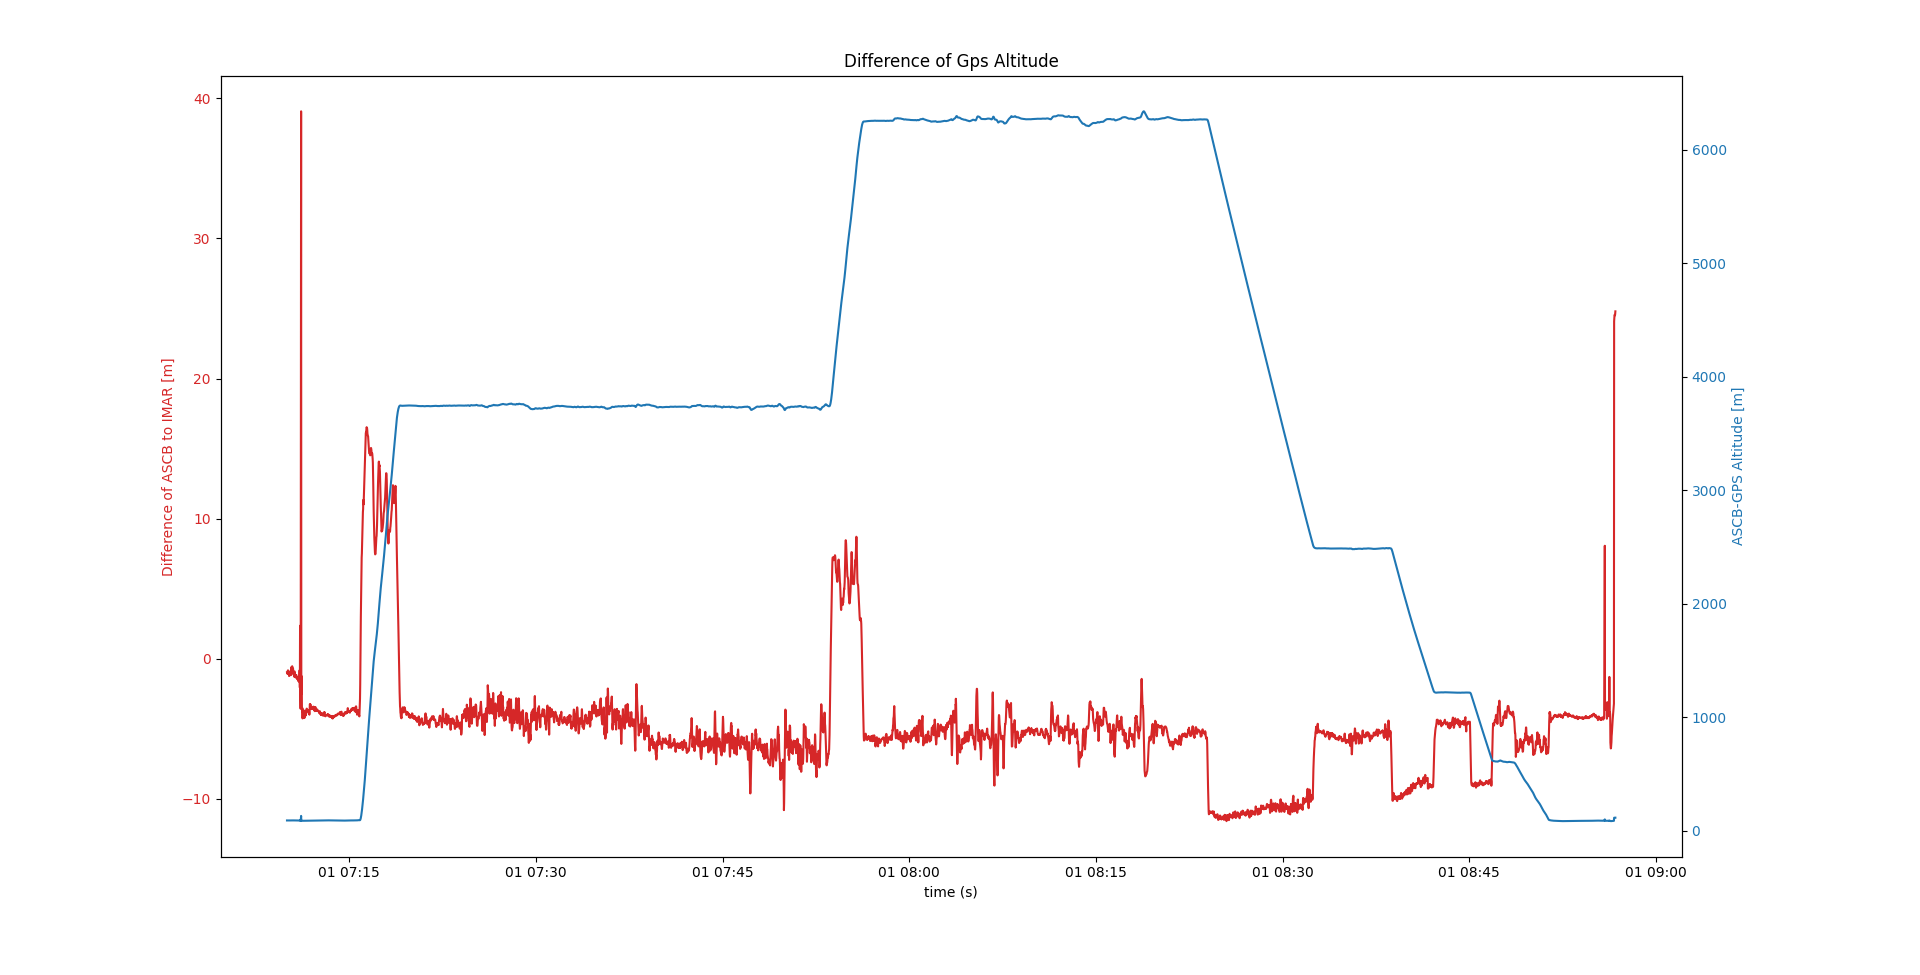
\includegraphics[width=.8\textwidth]{gps_difference_imar_ascb}
    \caption{Comparing the GPS sensors from the internal aircraft GPS (ASCB) to an experimentally installed GPS system (IMAR)}
    \label{fig:gps_diff}
\end{figure}

Another incurring deviation is investigating the ~40m/150ft offset for gps altitudes. Possible causes may be Uncorrected Ellipsoid gnss altitudes. However, this appears unlikely since generally the offset in the region would be added and not subtracted [further investigation needed].


Difficulty diagnosing sensors without previous knowledge. limitations within sensor behaviour. Checks include: range, too much sensor movement, too few sensor movement.

Relative examinations possible for errors occuring for finite time within experiment but not if all of the experiment data is corrupt.

\paragraph{altitude comparison}

plot here:
-gps to gps
-gps to baro. Beta overlayed as well as Ma Number


some mean ground has to be found to crossreference the various altitudes.

For standardization. The SI-unit meters is used for altitudes.

In the first draft. The altitude is sampled with 1Hz for computational speed and since gnss update rates are updated in a similar frequency.

\paragraph{ Physical}

\paragraph{ GNSS}

The following briefly glosses over GNSS and does not delve into the technical details. it rather tries to present GNSS Systems as a black box and examines inputs and outputs.

Generally speaking, GNSS systems calculate position based on run times to satellites. For output GNSS systems return position values for the ellipsoid model of the earth. Since the difference between MSL and ellipsoid varies for up to 100m vertically based on the receivers positions on the earth. Mostly, the difference is in the 40-50m range in germany.

Explain here why orthometric and ellipsoid value differs (vector difference, cg)

GNSS-units work with geoid models to deliver an orthometric value. Different Geoid models have different drawbacks and resolutions. For aviation use, the World Geodetic System (WGS84) generally proposes a geoid model that is used. Within this works scope it is omitted to implement an existing geoid model into the software-loop to reserve this workload for a later time.


\section{Report Visualization}

Motivation:


An interactive data report is chosen for data analytics since it works more efficiently and rather follows the paradigma of a single source of truth since it allows for dynamic updates and thus does not represent a data source in itself but rather view on the source.


Requirements:
needs to be able to quickly gain an overview over state of sensors. Details can be looked up later. UX-centric design.
Level1: Quickly see if many sensors are missing
Level2: Identify outliers

\subsection{Visualization}

\paragraph{of missing parameter list}
After monitoring, a list of missing parameters is generated. To show and detect this info quickly, a speed gauge style display is chosen to display this scalar value.

\paragraph{Displaying notable occurences of single sensor examination}
To quickly get an overview of missing parameters, a timeline graph is implemented, showing cumulative errors over the flight. This allows a quick overview over all parameters.


Possible features: implement altitude graph later to contextualize sensor behaviour.

\paragraph{Examining sensor interactions}

whole flight: occurences
Single sensor: mean value, residual, stdev


%\subsection{ Upload of JSON to stash}


%\subsection{ Check for errors}
It shows that while conservatively chosen ranges do not indicate many occurences, tighter limits enable more detailed monitoring.

\subsection{Adapt sensitivity and algorithms (balance false positives)}

The validation loop is driven by previously known error types (See OneNote Sensor Errors)


\section{Conclusion}

This parameter showed the methods used and the considerations made for the implementation of this SHM. Various methods and approaches were implemented to check for sensor faults. Next to the straight implementation, focus was put into developing solid interfaces to ease further implementation of future methods of fault detection. This applies for Levels 1, 2 as well as 3 which in this work was only minimally implemented to allow this prototype to see the light of day.





